%%%%%%%%%%%%%%%%%%%%%%%%%%%%%%%%%%%%%%%%%%%%%%%%%%%%%%%%%%%%%%%%%%%%%%%%%%%%%%%%%%%%%%%%%%%%%
% 																	INTRODUCTION																						%
%%%%%%%%%%%%%%%%%%%%%%%%%%%%%%%%%%%%%%%%%%%%%%%%%%%%%%%%%%%%%%%%%%%%%%%%%%%%%%%%%%%%%%%%%%%%%

%%%%%%%%%%%%%%%%%%%%%%%%%%%%%%%%%%%%%%%%%%%%%%%%%%%%%%%%%%%%%%%%%%%%%%%%%%%%%%%%%%%%%%%%%%%%%
% 															Chapter Introduction  																			%
%%%%%%%%%%%%%%%%%%%%%%%%%%%%%%%%%%%%%%%%%%%%%%%%%%%%%%%%%%%%%%%%%%%%%%%%%%%%%%%%%%%%%%%%%%%%%
\chapter{INTRODUCTION}


As robots move from more structured environments of laboratories to
unstructured environments like home and office, multiple challenges arises. One
of the challenges which arise is location of object in less structured and more
uncertain environments. This challenge gave birth to the probabilistic mapping
of the location of the objects in the environment, which enables estimating the
object location based on last seen information of the object. Some authors have
made effort to obtain information about the world dynamics and proposed
representations that model the object dynamics explicitly. This representation
show potential improvement in search of objects in highly dynamic environment.
However, as robots tend to achieve long term autonomy, a new challenge appeared
that the object locations in natural environment are subject to change in a
particular pattern. Although the probabilistic state estimation of objects can
deal with changes in the location of objects, their approach is rooted in
making conclusions based on the last seen location. This approach is good for
estimating the location of object in a world model. But it does not consider the
information available based on the movement of the object for predicting the
object location. This information of the current state if recorded then analysis
can be run on the object location to understand the mobility pattern in the
object location over time. Modelling this object mobility pattern will help in
predicting the object location in the environment. The prediction of location
will further enhance the search of objects. 

In classical object search, the search is on a generic home which causes the learning of the object location to be finite. Whereas the object search problem in real life is a continuous learning process which
never stops. Unlike the classical object search,  the proposed spatio-temporal object location learning is a daily
task which the robot has to carry out along with its daily routine. A typical
spatio-temporal object location learning will consist of repeated observations
of different objects in the environment spread throughout the robot's
operational time. Based on the observations the object model will be generated and updated. The learned model will then be used to predict the searched object location thus reducing the search time.

The generic home scenario, in classical object search doesn't take into account the differences in object locations from home to home. Based on practical experience we know that the even though homes have same base structure in space but the usage of the space is based on the user preferences. Each home is different from other home because of the humans which reside in them use it according to their likes. The proposed model will try to learn these user preferences in each home. So rather than learning object locations in a generalized home the proposed model shall learn object locations in a specific home.




\begin{figure}[htp]
\centering
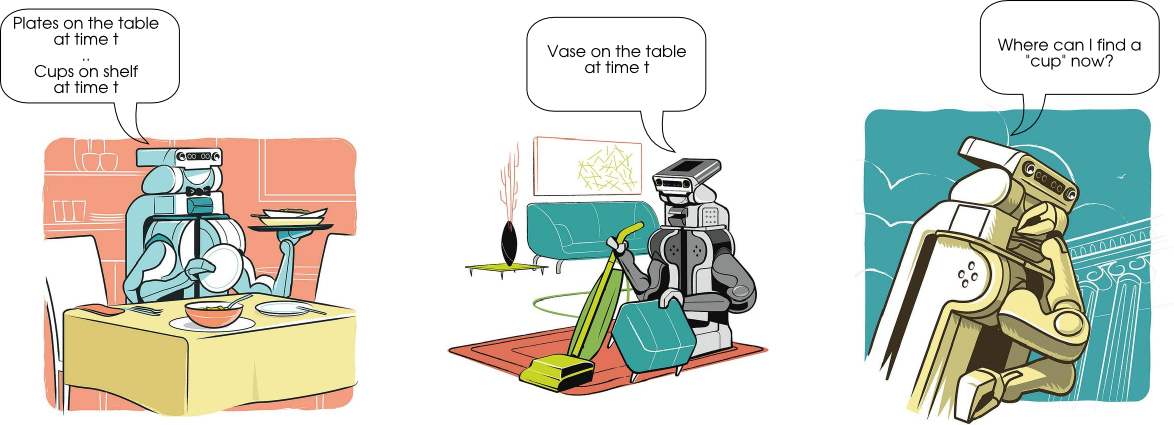
\includegraphics[scale=0.4]{pictures/scenario.png}
\caption{Robot recording perceived objects location and time. Based on the
recordings robot making prediction on the location of the cup for current time
Images courtesy : \url{https://www.flickr.com/photos/willowgarage} }
\label{scenario}
\end{figure}

Consider a domestic robot which has been placed in a home environment with a known map
and semantic information of the different locations in the home. The domestic robot while doing its daily activities 
makes a record of the objects seen in the environment with
their location and time. Now the robot has been asked to bring the coffee mug
of the user.
The robot has to make a decision which part of the home it has to go to look for
the coffee mug.
The robot can make this decision based on the previous observations of the 
location of the coffee mug.
The robot using the previous observations and the time of those observations 
makes a prediction about where the coffee mug can be found at the current time.
Based on previous observation it can be
inferred that the coffee mug is usually found in any of the following three location
dishwasher/platform/cupboard. Assuming that the time now is morning, from
previous observations it can be found that the coffee mug was always found  in the
dishwasher. The above example illustrate the main aspects of object location
prediction we wish to capture in our work.


The model needs to capture two main
elements; first that objects in a human environment are not placed randomly but
usually have a certain set of places where they are placed.
These places of object placement differ from home
to home. These object locations entirely depends on the users preferences.  
Second, that human behaviour is related to time i.e. Humans have daily routines  and the object locations are influenced by these routines.
Thus human behaviour not only  has a spatial behaviour but also has a temporal behaviour.
The model will reason on both user preference of the object location and the
object-time relation.



% section  (end)
